


\section{Credibly and empirically assessing risks}

The first area of research ethics that can be addressed with better practices is risk assessments. There is widespread consensus that research should not put participants at an unjustifiable risk of harm \citep{apsa2020ethics}. There is also an increasing recognition that it should not put collaborators, particularly research implementers and academics living in violent contexts, at risk. In the social sciences, however, risk assessments are not always empirically rigorous and are almost never replicable. Although we go to enormous lengths to empirically validate other aspects of our research methodologies, the process of assessing risks for IRBs or funders is more likely to be based on general impressions. Risk assessments rarely make it into articles or online appendices, as documented in Section \ref{sec:meta}. 

It is difficult to overstate the harm that can be caused by inadequate or biased risk assessments. \citet{eck2020time} discuss a study in Ethiopia in which 20\% of female participants reported being beaten by their male partners because of their participation. \citet{baaz2019exploring} discuss a case in which militant groups tortured a research facilitator and killed his family member because of his participation in a research project. Risk assessments must be thorough enough that research involving such excessive harm is never carried out.  

Making risk assessments part of publications that use data collected from participants living in violent contexts could move us closer to the goal of minimizing minor harms  and never inflicting severe harm. For example, in a 2019 article that uses original survey data from a lab experiment conducted in Zimbabwe, author two discusses in the article and appendix how consultations with local collaborators and the quantitative data on state repression collected by domestic human rights monitors led her to assess that the risk of punishment for participation in the research was justifiably low \citep{young2019psychology}. In this case, the existence of a high quality Zimbabwean human rights monitor and established political polling enabled her to make that assessment with confidence. Others can question whether the documented risk assessment was sufficient -- and our point is exactly that the assessment should be reviewed by other scholars. We know anecdotally that other researchers are doing similar or better risk assessments in their own projects. However, when these are not reported in research outputs there are no common norms around risk assessments. If scholars expect that they need to document risk assessments in publications (and not just in IRB applications, which are almost never made public) it creates incentives for thorough and accurate assessments. 

\section{Measuring and mitigating the risk of distress and negative psychological outcomes}

The risk of distress, lasting negative affect, and other adverse psychological outcomes has rightfully become a major concern in violence research. ``Re-traumatization'' is often used as a shorthand by social scientists for various forms of distress. Yet the empirical basis for assessing and avoiding the risk of distress and other adverse psychological outcomes or any positive psychological benefits in political science research is surprisingly small.

Over the past 25 years trauma psychologists have taken an empirical approach to the risk of negative psychological and affective consequences of participation in research. Psychologists have embedded questions designed to assess the incidence and severity of different harms in instruments used with trauma survivors. This literature tends to separately consider the risk of emotional distress during the research procedures, and the risk of longer-term negative outcomes \citep{legerski2010risks}. Two systematic reviews on the risk-benefit ratio of participation in trauma research have concluded that while many participants do report harm, those harms are often offset by perceived benefits and in most studies regret is rare \citep{jaffe2015does, mcclinton2015adolescents}. Finally, though there have been few studies that use credible methods like randomized controlled trials to test for longer-term effects of research participation, one review concluded that there are few signs of long-term negative effects in research on trauma in psychiatry \citep{jorm2007participant}. 

There remain many open questions around the emotional and psychological risks of political science research. A first-order question is how well the empirical findings from psychology and psychiatry generalize to political science. Almost all of the studies in existing meta-analyses were conducted with American or European participants, while much political science research on violence is conducted outside of these ``WEIRD'' (Western, educated, industrialized, rich, and democratic) contexts \citep{henrich2010weirdest}. Second, open questions persist across fields. Are some sub-groups of participants more likely to experience severe or prolonged harms relative to others? What are the best ways to design questions or interview protocols so that the risk of mild distress is minimized, and severe harms are avoided? This should be a growing area of methodological innovation in the social and behavioral sciences. 

A second and complementary approach to minimizing the risk of negative psychological outcomes involves the provision of psychosocial support. It has become fairly common in political science to set up a psychosocial referral system for participants, however post-study referrals are often insufficient to protect participants from the potential negative impacts of research. In many contexts, quality services are unavailable or prohibitively costly. Furthermore, political science researchers often lack the training to identify culturally appropriate resources, so we may identify inappropriate resources or make errors when deciding who to refer for support. Finally, it is often impossible to determine whether psychological distress was caused by the research or not. Most fundamentally, providing assistance to people who have been harmed by a study is clearly inferior to avoiding that harm in the first place. 


We identify two low-cost practices that may reduce the risks of negative psychological outcomes among participants and fieldwork staff. First, more consistently measuring experiences of distress during interviews, and when possible, symptoms of negative psychological outcomes in the period following participation, would enable researchers to better understand and avoid these risks. In some cases we have asked interviewers to assess whether they think participants are experiencing distress \citep{young2019psychology}. 

In one of our Mexico studies -- a field experiment that involved three interviews and a community discussion -- we tracked PTSD symptoms over three rounds of measurement to test whether participants with symptoms reported higher levels of distress during the study, and whether PTSD symptoms were affected by participation in a small-group discussion about crime. We do not find evidence that participating in community discussion groups on crime led to an increase in PTSD symptoms \citep{baron2020lab}. The marginal cost of a few additional interview questions is small, as such questions can be added to the end of existing interviews or in the ``back-checking'' that is common in large-scale surveys. 

These experiences also left us with questions. Is it better to rely on research staff or participants themselves to assess research-related distress? To what extent might social desirability or performance pressure lead either group to under-report distress? More rigorous research is needed to develop and validate measures appropriate for social science research on violence. Having a body of evidence on harms and benefits would enable us to identify the practices that are least likely to have negative psychological consequences. This evidence could be quickly generated if questions about psychological distress were regularly embedded in research protocols.

Second, psychosocial support professionals can be enlisted at early stages in fieldwork to prevent and mitigate the risk of distress and more extreme negative reactions. Building on practices described in \citet{paluck2009deference}, in our qualitative study in Mexico we worked with a local trauma specialist and certified counselor to train our interviewers on how to identify and prevent severe distress. Additionally, this specialist provided interviewers with techniques to cope with secondary trauma, and served as a counseling resource during and after the fieldwork. For the field experiment involving discussion groups, we hired two counselors who regularly work with local survivors of violence as facilitators to ensure that our team had the skills and motivation to identify and avoid distress. In our case, these strategies were not costly: we offered the trauma specialist a \$200 honorarium, and the decision to hire counselors instead of standard research facilitators required no additional resources. In contexts where mental health professionals are scarce, it may still be feasible to have a mental health professional with experience in the cultural context review the research protocol or offer remote support. 



\section{Assessing whether consent is really informed}

The principle of respect for persons implies that people should be free to make an informed decision about participation in research. IRBs typically require a standard set of information to be provided: What tasks will participants perform? What are the potential risks and benefits? How will privacy be guaranteed? Potential participants in violence research are often told that the study involves sensitive topics, and that they might become upset. They have the chance to ask questions before they make a decision.  

Violence researchers could do more to assess the adequacy of the consent process. The main concern in the informed consent process is that participants have enough information to make a personal decision that they would be satisfied with if they had complete information. To this end, trauma researchers often include questions about regret regarding participation. In our research we have simply asked participants if they are happy or unhappy that they consented at various points in the study process, and what they are happy or unhappy about, in order to monitor the adequacy of the consent process. If the vast majority of participants say that they are happy with their decision, it suggests that the consent process is adequate.  

For the recent field experiment that we carried out in Mexico, we specified that if more than 5\% of participants were telling us that they were not happy, we would pause the study and retool the consent process to provide more information on the elements that unhappy participants were mentioning. After a first 20-minute interview, 0.6\% of participants regretted their participation. After a half-day community discussion and second 20-minute interview, 0.3\% expressed regret. By a final 20-minute follow-up interview, no participants expressed regret \citep{baron2020lab}.

Another empirical approach to assess informed consent involves asking participants factual questions about the consent process. The Afrobarometer surveys, for example, ask participants who they think the sponsor of the research is. Additional factual questions could test if and how participants understand important conditions of the consent process. Do participants understand that they can stop the interview or skip questions? Do participants see their participation decision as one over which they have individual autonomy, or do they experience it as determined by a local elite or relative? Ultimately, assessing the quality of the informed consent process should be an area of methodological development. 

\section{Monitoring the actual incidence of harms}

Actively monitoring for harms, particularly coercion or retribution associated with research participation, is arguably the most important and challenging of the four practices we discuss. Robust measurement of potential harms and management systems to quickly communicate information and adapt research protocols are obvious practices that could help researchers prevent potential harms. Reporting on observed harms is also an accepted standard in medical trials, and has been adopted as an item in the CONSORT reporting guidelines.\footnote{For more on the CONSORT group, see \url{http://www.consort-statement.org/}.} It would also build on recent efforts to measure and report harms to research collaborators in authoritarian settings \citep{grietens2019repressive}. However, the rate of unintended consequences and how they were monitored is rarely reported in social science research outputs. 

Researchers can monitor unintended consequences in follow-up surveys with participants or through debriefs with research staff. In our Mexico experiment we asked participants in the follow-up calls whether they experienced retaliation, emotional distress, or any other negative consequence due to participation in discussion groups on crime and responding to crime. However, not all research designs permit this kind of follow-up. In particular, this type of follow up cannot be done for anonymous studies. In cases where we could not directly follow-up with participants, we have relied on local research partners to monitor major risks.  This type of monitoring is likely to pick up major events of retaliation, but less likely to detect emotional distress and other private harms. 

Monitoring harms can enable researchers to modify or stop research projects if early data shows that research-related harm is occurring. If research has unintended consequences, transparency is the fastest way that violence researchers as a field can learn about them and prevent them in future studies. In addition, reporting monitoring practices and incidences of harms enables ethical practices to become a more robust part of the peer review process to create incentives for researchers to use appropriate methods in their research.

\section{Assessment of current reporting practices}\label{sec:meta}

How transparent are research methods related to ethics in violence research involving human participants? We had a team of five undergraduate and Masters-level research assistants code 172 research articles on political violence that involved human participants published between 2008 and 2019 in six influential political science journals. Our research assistants used a coding guide to identify any mention of research ethics in six categories in the article or appendix: IRB review, risk assessments, consent processes, harms observed, risk to research teams, and any other information related to ethics. Each article was double-coded, and the inter-rater reliability scores varied from 0.84 for the undefined ``other'' category to 0.95 for an indicator of whether the IRB number was reported in the publication.

A few points are worth keeping in mind when interpreting this review. First, the RAs were given very inclusive coding guidelines: if an article or appendix mentioned anything about risks associated with the research project, it was coded as ``yes'' in the risk assessment category. Similarly, if it mentioned anything about informed consent (including just a passing comment that consent was obtained) it received a ``yes'' in the informed consent category. Thus, this is not an assessment of whether existing research is employing the practices we recommend. Second, this is not an analysis of whether existing research is violating ethical practices. We believe that many researchers are doing more to adhere to ethical principles than they report in their articles and appendices. Our goal is to assess the extent to which basic elements of research transparency around ethics have been voluntarily adopted in a setting where the stakes of ethical practices are high. 

In general, information related to ethics is rarely reported in publications. Figure \ref{fig:practices} shows the proportion of all articles based on research with human participants on violence published from 2008-2019 that provided at least some discussion of our six areas of transparency. 


\begin{figure}[hbt!]
    \centering
    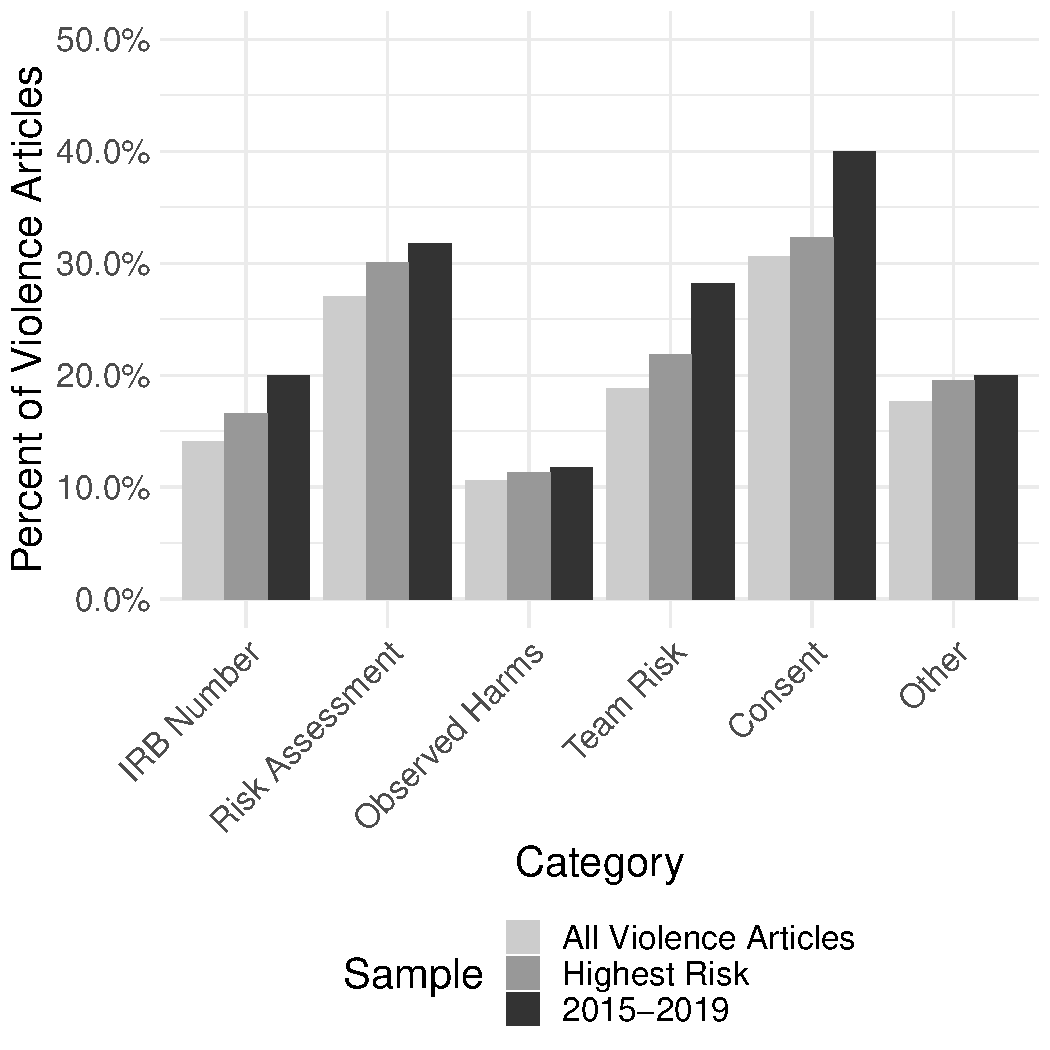
\includegraphics[width=0.5\textwidth]{Pct_Transparent.pdf}
    \caption{Percent of articles that study political violence with human participants that mention types of research ethics considerations, 2008-2019}
    \label{fig:practices}
\end{figure}

The first column in each category shows the percent of all identified violence articles with human participants that provides an IRB number, discusses risks considered, reports on observed harms, discusses risk to research team members, gives details of the consent process, or provides any other discussion of ethics. In total, just 11\% of articles report anything related to observed harms, and 31\% mention a consent process. Again, it is important to keep in mind that we coded these categories as ``yes'' if an area of ethics was even mentioned in passing -- a much smaller proportion of the articles provide enough information to let readers assess whether the practices were adequate. The percentages of articles mentioning ethics are slightly higher when we exclude seemingly low-risk research, such as public opinion surveys on foreign conflicts or research on less sensitive topics like clientelism in non-democratic regimes (Bar 2). Finally, Bar 3 shows that articles published in the last five years generally has more discussion of research ethics, particularly around risk to research team members and the consent process. Nevertheless, in all cases it is clear that discussion of research ethics in publications is far from the norm. 

\section{Conclusion}

There are no silver bullets in research in violent contexts. We have suggested a few practical steps that can be taken to help researchers better adhere to the principles we have widely accepted as a research community. At their core, these suggestions are practices that increase the ability of researchers to monitor their own projects for implementation failures and unintended consequences around research ethics, and to increase the transparency of decisions around ethics. They complement a recent list of questions on ethics that reviewers should ask for research in violent contexts \citep{cronin2018ethics}, a suggested template for ``ethics appendices'' recently proposed for randomized controlled trials \citep{asiedu2021call}, and updated submission practices at the American Political Science Review (APSR). We also see our suggestions as being in line with the ethics guidelines adopted by the APSA \citep{apsa2020ethics}. In particular, these guidelines call for researchers to identify and justify potential harms in presentations and publications. There is no reason that research ethics should not be an area of methodological innovation and research, just as other forms of research transparency have become in recent years as scholars have developed better methods for detecting p-hacking, pre-registration, and replication \citep{humphreys2013fishing, simonsohn2014p, open2015estimating}. 
 
In no way do these practices make ethical decisions in violent contexts easy. Is it ever worth putting a participant at some risk of harm in order to learn something about political violence? Can we ever assess risks with sufficient confidence to make research design decisions, given that violence changes unpredictably and is often shrouded in uncertainty? 
 These questions weigh ethical imperatives against each other -- the goal to use research to tackle the most important problems that society faces, the imperative to do no harm, and the need to take action with imperfect information. But making the decisions more evidence-based and transparent through methodological innovations might help us move closer to the best balance of these principles. 




\begin{acknowledgement}
This note draws on research conducted with a number of collaborators, including Omar Garc\'{i}a-Ponce, Adrienne LeBas, Alexander Noyes, and Thomas Zeitzoff. We also learned significantly from research implementers in Mexico and Zimbabwe. These projects benefited from funding from the National Science Foundation, U.S. Institute of Peace, and International Peace Research Foundation. We thank Cyril Bennouna, Graeme Blair, Robert A. Blair, Dara Kay Cohen, Jennifer Freyd, Macartan Humphreys, Sabrina Karim, Emilia Simison, Tara Slough, participants at the Brown-MIT Development Workshop, and two anonymous reviewers for invaluable feedback.
\end{acknowledgement}